%\documentclass[10pt,landscape,handout]{beamer}
%\documentclass[10pt,landscape,draft]{beamer}
\documentclass[10pt,landscape,xcolor=dvipsnames]{beamer}


% Be able to directly input German Umlauts etc.
%\usepackage[latin1]{inputenc}

% Font encoding:
\usepackage[T1]{fontenc}
\usepackage{lmodern}
\usepackage[utf8]{inputenc}
\usepackage{german}
\usepackage{ragged2e}
\usepackage{epstopdf}
\usepackage{setspace}
\usepackage{graphicx}

\definecolor{shadecolor}{rgb}{0.8,0.8,0.8}
\definecolor{white}{rgb}{1.0,1.0,1.0}

\newif\ifplacelogo % create a new conditional
\placelogotrue

\usepackage{units}
\usepackage[absolute,verbose,overlay]{textpos}

\newcommand{\poslogo}{%
  \setlength{\TPHorizModule}{364pt}
  \setlength{\TPVertModule}{273pt}}
  



% setup beamer style to use TUDo Theme
\mode<presentation>
{
  \usetheme{TUDortmund}
}

% Include intermediate TOCs automatically.
% Completely pointless for these slides, however
%\AtBeginSection[]
%{
%  \begin{frame}<beamer>
%    \frametitle{\"Ubersicht}
%    \tableofcontents[currentsection]
%  \end{frame}
%}

\setbeamertemplate{navigation symbols}{}
\setbeamertemplate{}[frame number] 
%%%%%%%%%%%%%%%%%%%%%%%%%%%%%%%%%%%%%%%%%%%%%%%%%%%%%%%%%%%%%%%%%%%%%
%%% Basic information
%%%%%%%%%%%%%%%%%%%%%%%%%%%%%%%%%%%%%%%%%%%%%%%%%%%%%%%%%%%%%%%%%%%%%


\title[]{Transmissionselektronenmikroskopie}

\subtitle{Seminarvortrag}

\author{Markus Stabrin}

\institute[Fakult\"at f\"ur Physik, TU Dortmund]{Fakult\"at f\"ur Physik\\ Technische Universit\"at Dortmund}
\date{11. Dezember 2014}



\begin{document}
\setlength{\parskip}{1mm}

%%%%%%%%%%%%%%%%%%%%%%%%%%%%%%%%%%%%%%%%%%%%%%%%%%%%%%%%%%%%%%%%%%%%%
%%% Title
%%%%%%%%%%%%%%%%%%%%%%%%%%%%%%%%%%%%%%%%%%%%%%%%%%%%%%%%%%%%%%%%%%%%%

% use logo for title slide

% \logo{\ifplacelogo \includegraphics[width = 5cm]%{pic/Bild30}\hspace{3.75cm}\fi}


% slide options are: alignment: c(enter) or t(op), label
%\afterpage{%
\begin{frame}[c,label=titlepage]
  \titlepage
\end{frame}

% \begin{frame}
%   \frametitle{Inhaltsübersicht}
% 	\begin{minipage}{6cm}
%   \setcounter{tocdepth}{2}
% 	\footnotesize{
%   \tableofcontents}
% 	\end{minipage}
% 	\begin{minipage}{3cm}
		
% 	\begin{figure}
% 		\centering
% 			\includegraphics[width=5cm]{pic/Bild1.png}
% 	\end{figure}
	
% 	\end{minipage}
% \end{frame}

%%%%%%%%%%%%%%%%%%%%%%%%%%%%%%%%%%%%%%%%%%%%%%%%%%%%%%%%%%%%%%%%%%%%%
%%% Overview
%%%%%%%%%%%%%%%%%%%%%%%%%%%%%%%%%%%%%%%%%%%%%%%%%%%%%%%%%%%%%%%%%%%%%

% turn off logo for remaining slides (just draws away focus from content)
%\logo{}

%\begin{frame}[t, label=overview]
  %\frametitle{\"Ubersicht}
  %\setcounter{tocdepth}{2}
  %\tableofcontents
%\end{frame}


%%%%%%%%%%%%%%%%%%%%%%%%%%%%%%%%%%%%%%%%%%%%%%%%%%%%%%%%%%%%%%%%%%%%%
%%% Global structure is declared through the usual section and 
%%% subsection environments. Starred sections will not appear in the 
%%% auto-generated TOCs.
%%%%%%%%%%%%%%%%%%%%%%%%%%%%%%%%%%%%%%%%%%%%%%%%%%%%%%%%%%%%%%%%%%%%%

\section[EPA]{Einzelpartikelanalyse} % (fold)
\label{sec:einzelpartikelanalyse}
\subsection*{subsection name} % (fold)
\label{sub:subsection_name}

% subsection subsection_name (end)
\begin{frame}
	\frametitle{Einzelpartikelanalyse}
	\begin{figure}
		\includegraphics[width = 7cm]{pic/epa2.png}
	\end{figure}
	\begin{figure}
		\includegraphics[width = 8cm]{pic/epa_all.png}
	\end{figure}
\end{frame}

\begin{frame}
	\frametitle{Einzelpartikelanalyse}
	\begin{block}{Auswahl und Klassifizierung}
		\begin{itemize}
			\item Manuelle Auswahl der Partikel
			\item Gleiche Ausrichtung aller Partikel
			\item Klassifizierung
		\end{itemize}
	\end{block}
	\centering
	\begin{minipage}{3.5cm}
		\begin{figure}
			\includegraphics[width = 3.5cm]{pic/k_c_1.png}
		\end{figure}
	\end{minipage}
	\begin{minipage}{3.5cm}
		\begin{figure}
			\includegraphics[width = 3.5cm]{pic/k_c_2.png}
		\end{figure}
	\end{minipage}
	\begin{minipage}{3.5cm}
		\begin{figure}
			\includegraphics[width = 3.5cm]{pic/k_c_3.png}
		\end{figure}
	\end{minipage}
\end{frame}

\begin{frame}
	\frametitle{Einzelpartikelanalyse}
	\begin{block}{Erste Rekonstruktion}
		\begin{itemize}
			\item Klassensummen als Projektionen
			\item Startmodell aus Gaußschem Rauschen
			\item Kreuzkorrelation
		\end{itemize}
	\end{block}
	\begin{figure}
		\includegraphics[width = 5.5cm]{pic/recons.png}
	\end{figure}
\end{frame}

\begin{frame}
	\frametitle{Einzelpartikelanalyse}
	\begin{block}{3D Refinement}
		\begin{itemize}
			\item Simulation von 2D Projektionen
			\item Vergleich und Ausrichtung der Partikel
			\item Radon Transformation
		\end{itemize}
	\end{block}
	\begin{figure}
		\includegraphics[width = 8cm]{pic/epa1.png}
	\end{figure}
\end{frame}

\begin{frame}
	\frametitle{Einzelpartikelanalyse}
	\begin{figure}
		\includegraphics[width = 11cm]{pic/radon.jpg}
		\hspace{3cm}
	\end{figure}
	\vspace{3cm}
\end{frame}

\begin{frame}
	\frametitle{Einzelpartikelanalyse}
	\begin{figure}
		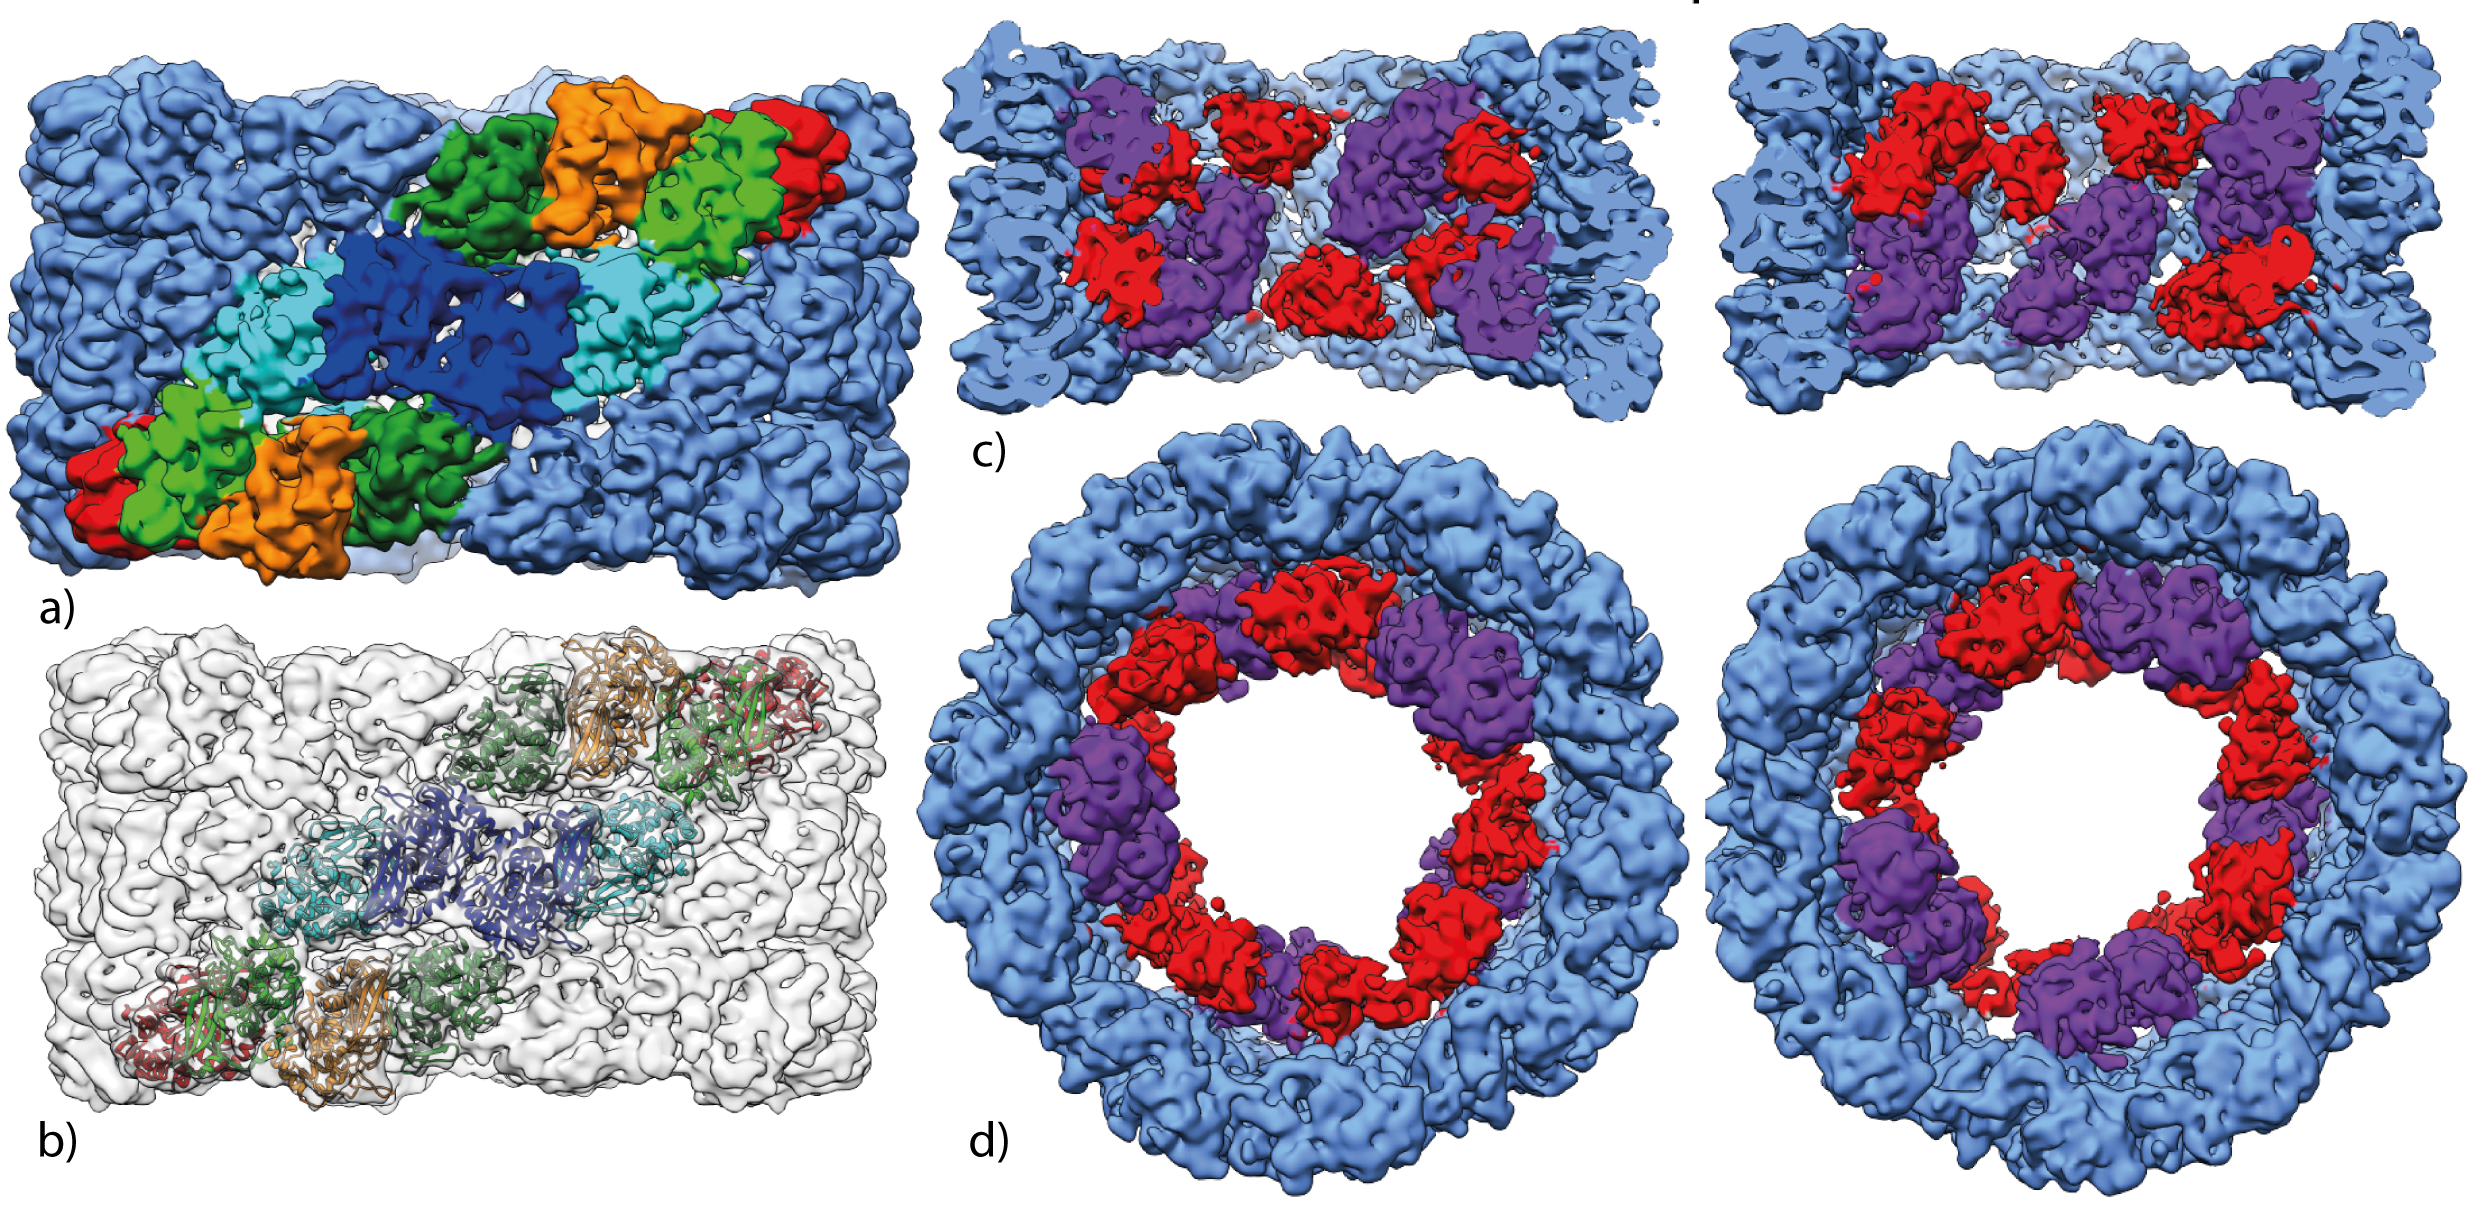
\includegraphics[width = 11cm]{pic/diezwei.png}
	\end{figure}
\end{frame}


% 

\section{Einleitung - Ein wenig Biologie}
\subsection{Was ist Denaturierung?}
\begin{frame}
  \frametitle{Was ist Denaturierung?}
	\begin{block}{Denaturierung}
	\begin{itemize}
	\item Aufbruch von Bindungen
	\item Strukturelle Veränderung des Biomoleküls ab der Sekundärstruktur
	\item Veränderung/ Verlust der Funktion und spezifischer Eigenschaften
	\item Mögliche Ursachen: Temperaturerhöhung, Änderung des pH-Werts oder der Salzkonzentration, Strahlenschäden, Chemikalien
	\end{itemize}
	\end{block}
		\begin{minipage}{3.5cm}
		\centering
\begin{figure}[h]
	\centering
		\includegraphics[width=3cm]{pic/ei.jpg}
\end{figure}
	\cite{EI14}
\end{minipage}
\begin{minipage}{3.5cm}
		\centering
\begin{figure}[h]
	\centering
		\includegraphics[width=2cm]{pic/fieber.jpg}
\end{figure}
	\cite{TH14}
\end{minipage}
\begin{minipage}{3.5cm}
		\centering
\begin{figure}[h]
	\centering
		\includegraphics[width=3cm]{pic/quelle.jpg}
\end{figure}
	\cite{QU14}
\end{minipage}

\end{frame}


\begin{frame}
\frametitle{Schädigung? - Lebensnotwendig!}
\vspace{0.1cm}
\centering
\small Denaturierung ist ein notwendiger Bestandteil lebenserhaltender Prozesse.
Verwendung für Bio-Chemische-Technologien, wie PCR.
\vspace{0.3cm}
  
\centering
		\begin{minipage}{7cm}
		\centering
\begin{figure}[h]
	\centering
		\includegraphics[width=6.5cm]{pic/transkription.jpg}
\end{figure}
	\cite{TK14}
	Transkription
\end{minipage}
\begin{minipage}{5.0cm}
		\centering
\begin{figure}[h]
	\centering
		\includegraphics[width=4.5cm]{pic/Replikation.png}
\end{figure}
	\cite{RK14}
	Replikation
\end{minipage}
\end{frame}

\subsection{Struktur der DNA}
\begin{frame}
\frametitle{Struktur der DNA}
		\centering
\begin{figure}[h]
	\centering
		\includegraphics[width=10cm]{pic/Backbone.jpg}
\end{figure}
	\cite{BIO09}
\end{frame}

\begin{frame}
\frametitle{Struktur der DNA}
\begin{figure}[h]
	\centering
		\includegraphics[width=9cm]{pic/Basen.jpg}
\end{figure}
\centering
	\cite{BIO09}
Stickstoffbasen\\
	\vspace{1cm}
Die drei Bestandteile des Nukleotids geben sowohl die Funktion der DNA, wie auch die Struktur der Doppelhelix vor.\\
\vspace{0.5cm}
Ohne die Elemente P, O, N, C und H ist kein Leben möglich.
\end{frame}

\begin{frame}
\frametitle{Struktur der DNA}
\vspace{0.5cm}
\centering
\begin{minipage}{4.5cm}
\begin{figure}[h]
	\centering
		\includegraphics[width=4cm]{pic/Chemical.jpg}
\end{figure}
\centering
	\cite{BIO09}
	\end{minipage}
	\begin{minipage}{4.5cm}
\begin{figure}[h]
	\centering
		\includegraphics[width=2.3cm]{pic/Ribbon.jpg}
\end{figure}
\centering
	\cite{BIO09}
	\end{minipage}
	\centering
	
	\vspace{0.3cm}
	\small Entscheidend für die Struktur der Doppelhelix sind Wasserstoffbrücken und Stapelwechselwirkungen benachbarter BP.\\
	%%Bei der Denaturierung werden nur H-Brücken aufgebrochen.
	\end{frame}
	
	\begin{frame}
	\frametitle{Stapelwechselwirkungen}
	\small
Phosphatrückgrat: hydrophil \& Basen: hydrophob\\
	$\Rightarrow$ Um das Wasser aus dem Zwischenraum zu verdrängen, "`stapeln"' sich die Basen dicht auf einander.
	\begin{itemize}
	\item Es handelt sich um eine ungerichtete WW
	\item Verringerung der Kontaktfläche zwischen Wasser und lipophiler Schicht \\ $\Rightarrow$ Entropiegewinn
	\item Chemisch durch eine WW der $\pi$-Elektronensysteme der beiden Basen zu verstehen.
	\item Typische Eigenschaften von planaren, (quasi-)aromatischen Strukturen.
	\item Stapel-WW ist sequenzabhängig, am schwächsten ist AT-AT	und GC-GC am stärksten (TD stabiler)
	\end{itemize}
	\begin{block}{}
	Bei der Denaturierung werden zuerst die dominierenden Stapel-WW überwunden, anschließend die schwächeren H-Brücken aufgebrochen.
	\end{block}
	
	\end{frame}
	
	
	
	\begin{frame}
	\poslogo
	\begin{textblock}{1}(0.488,0.005)
   \includegraphics[width=1cm]{pic/hut.png}
  \end{textblock} 
	\frametitle{Watson-Crick-Modell}
	\begin{block}{Ein Durchbruch für die Strukturaufklärung}
	\begin{itemize}
	\item 1953 veröffentlichten Watson und Crick einen kurzen Artikel über die rechtshändige, helikale Struktur der DNA
	\item 1962 erhielten Watson, Crick \& Wilkins für ihr räumliches Modell der DNA den Nobelpreis für Medizin
	\end{itemize}
	\end{block}	
	\vspace{0.2cm}
	\begin{itemize}
	\item Theorien wurden aus Röntgenaufnahmen abgeleitet.
	\item Vor der Veröffentlichung wurden Verwicklungen von 3 Strängen postuliert.
	\end{itemize}
	Watson \& Crick erkannten unteranderem, dass 
	\begin{itemize}
	\item nur A--T und G--C binden.
	\item eine Desoxyribose vorhanden sein muss.
	\item H-Brücken die entscheidende WW sind.
	\end{itemize}
	\end{frame}

% 
\section{Die Fragen der Denaturierung}
\subsection{Schmelzkurven - Denaturierung durchleuchtet}

\begin{frame}
\frametitle{Schmelzkurven}
\begin{block}{Schmelztemperatur $T_\text{m}$}
Temperatur bei der die Hälfte der DNA denaturiert ist.
\begin{itemize}
\item Abhängig von der DNA-Sequenz
\item Liegt zwischen 50-100 $^\circ$C
\end{itemize}
\end{block}
\centering
\vspace{0.5cm}
Experimentell aus Schmelzkurven bestimmbar.
\vspace{0.5cm}
\frametitle{Schmelzkurven}
\begin{block}{Schmelzkurve}
Relative Absorption $\theta$ bei meist 260 nm als Funktion der Temperatur.\\
\begin{itemize}
\item Kummulatives Schmelzprofil :  $1-\theta(T)$
\item Differentielles Schmelzprofil : $-\frac{\text{d}\theta}{\text{d}T}$
\end{itemize}
\end{block}
\end{frame}

\begin{frame}
\frametitle{Schmelzkurven}
\begin{minipage}{5.2cm}
\begin{figure}[h]
	\centering
		\includegraphics[width=5.0cm]{pic/Schmelz.jpg}
\end{figure}
\centering
\tiny\cite{GOT83}
\end{minipage}
\begin{minipage}{5.0cm}
\small{
\begin{itemize}
\item Schmelzkurven zeigen reproduzierbare Feinstruktur
%\item Einander folgende kooperative Teilübergänge
\item Schmelzregionen $\approx$ kBP denaturieren in Intervallen von 0,3-0,5 $^\circ$C
\item Schärfere Struktur für kurze DNA
\end{itemize}}
\end{minipage}
\begin{block}{}
\begin{itemize}
\item Feinstruktur durch Schmelzen kooperativer Schmelzregionen (Loops)
\item Öffnung eines Loops beeinflusst die Stabilität benachbarter Loops
\item Minimale Fluktuationen der BP verändern die Feinstruktur signifikant 
\end{itemize}
\end{block}
\centering
Die Öffnung von kooperativen Loops kann mittels Elektronenmikroskopie verfolgt werden.
\end{frame}


\subsection{Motivation}
\begin{frame}
\frametitle{Motivation}
\vspace{0.8cm}
\setstretch{1.5}
\begin{itemize}
\item Prozess der enzymatischen Denaturierung noch nicht verstanden
\item Verständnis thermischer Denaturierung wäre ein erster Schritt
\end{itemize}
\vspace{0.6cm}
\begin{figure}[]
	\centering
		\includegraphics[width=1\textwidth]{pic/Fragen.JPG}
\end{figure}
\end{frame}

\subsection{Fortschritt im Laufe der Zeit}
\begin{frame}
\frametitle{Fortschritt im Laufe der Zeit}
\setstretch{1.5}
\begin{tabbing}
 \textcolor{YellowGreen}{1953}$\qquad$\= Veröffentlichung Watson \& Crick zur DNA Doppelhelix\\
\textcolor{YellowGreen}{1960er}\> Beobachtung erster Schmelzkurven mit Feinstruktur\\
\textcolor{YellowGreen}{1970er}\> Goldene Ära der Schmelzstudien\\
\textcolor{YellowGreen}{1970}\> Erste DNA-Sequenzierungs Methoden\\
\textcolor{YellowGreen}{1977}\> Poland-Fixmann-Freire Algorithmus\\
\textcolor{YellowGreen}{1990er}\> Computertechnik und das WorldWideWeb\\
\textcolor{YellowGreen}{1990er}\> DNA Sequenzierung: schneller und günstiger\\
\textcolor{YellowGreen}{2000} \>Bestimmung der Ordnung des Phasenübergangs\\
\textcolor{YellowGreen}{2004} \>Erste Entschlüsselung des menschlichen Genoms
\end{tabbing}
\end{frame}
% 
\section[Theoretische Modelle]{Die Theorie der Denaturierung}
\setstretch{1}

\subsection{Grundlagen}
\begin{frame}
\frametitle{Grundlagen der Standardmodelle}
Die meisten Modelle bauen auf einem Basismodell ähnlich dem Isingmodell von B. H. Zimm auf (1960).\\
\vspace{0.4cm}
Verwendete Annahmen
\begin{itemize}
\item DNA als 1D Gitter aus N BP
\item H-Brücken zwischen komplementären Basen
\item Hydrophobe/ Stapelwechelwirkung zwischen nächsten Nachbarn
\item Zwei Zustände für BP: gebunden / ungebunden
%\item Berücksichtigung der Konfigurationsentropie und des Disszoziationsgleichgewichts
\end{itemize}
\end{frame}

\subsection{Basenpaar-Modell}
\begin{frame}
\frametitle{Basenpaar-Modell}
\begin{minipage}{5.2cm}
\setstretch{1}
\begin{figure}[h]
	\centering
		\includegraphics[width=5.0cm]{pic/BPModell.jpg}
\end{figure}
\centering
\tiny\cite{GOT83}
\end{minipage}
\begin{minipage}{5.0cm}
\setstretch{1}
\small{
\begin{itemize}
\item Nummerierung der BP vom 5' zum 3' Ende
\item Beschreibung durch einen N-Dimensionalen Vektor $\vec{c}$ 
\item BP: offen 0, geschlossen 1
\end{itemize}
}
\end{minipage}
\vspace{0.2cm}
\setstretch{1}
Zustandsumme $Z_c$ ist das Produkt der Stapilitätsparameter $s_k$ und Loop-Gewichtungsfaktoren $\sigma_l$.
Faktoren werden nach folgenden Regeln verwendet.
\begin{itemize}
\item Gebundenes k-tes BP $\Rightarrow\, s_k$
\item Innerer Loop mit l ungebundenen BP $\Rightarrow\, \sigma_l$
\item Gewichtung 1 für die Enden der Kette (keine freie Energie).
\end{itemize}
\end{frame}

%\begin{frame}
%\frametitle{\large Freie Energie und Wahrscheinlichkeiten}

%%%%%%%%%%%%%%%%%%%%%%%%%%%%%%%%%%%%%%%%%%%%%%%%%%%%%%%%%%%%%%%%%%%%%%%%%%%%%%%%%%%%%%%%%%%%%%%%%%%%%%%%%%%%%%%%%%POSITION DER FOLIE?? ETWAS NICHTSSAGEND?\\
%Freie Energie
%\begin{align*}
%F_c=-\text{R}T\ln(Z_c)
%\end{align*}
%Wahrscheinlichkeit der Konfiguration $c$
%\begin{align*}
%P_c=\frac{Z_c}{\sum Z_c}
%\end{align*}

%Helizität einer Doppelhelix mit $N_c(1)$ gebundenen BP
% \begin{align*}
%\Theta= \frac{\sum N_c(1) Z_c}{\sum Z_c}
%\end{align*}
%\end{frame}


\subsection{Stacking-Modell}
\begin{frame}
\frametitle{Stacking-Modell}
\small Die dominante, strukturgebende WW der DNA ist die Stacking-WW \\
\centering{ $\Rightarrow$ anpassen des Modells.}\\
\begin{minipage}{5.2cm}
\begin{figure}[h]
	\centering
		\includegraphics[width=5.0cm]{pic/STModell.jpg}
\end{figure}
\centering
\tiny\cite{GOT83}
\end{minipage}
\begin{minipage}{5.0cm}
\small{
\begin{itemize}
\item Jedem BP Doublet wird ein Stabilitätsparamter zugewiesen
\item Beschreibung durch einen N-1-Dimensionalen Vektor $\vec{c}$
\item WW zwischen Doublet $\hat{=}$ stacked
\item stacked 1 / unstacked 0
\end{itemize}
}
\end{minipage}

\begin{flushleft}
Regeln der Zustandssumme können übernommen werden, mit
\begin{itemize}
\item $l$ = \# unstacked Doublets= \# offene BP + 1
\item $k$ = Doublet aus k-tem und (k+1)sten BP
\end{itemize}
\end{flushleft}
\end{frame}

\subsection{Das Parameterproblem}
\begin{frame}
\frametitle{Das Parameterproblem}

\textbf{Stabilitätsparameter} des Basenpaars MN
\begin{align*}
s_k=s_{MN}=\exp\left(-\frac{\Delta H_{MN}-T\Delta S_{MN}}{\text{R}T}\right)
\end{align*}
\begin{itemize}
\item Die Entropie $\Delta S_{MN}$ und Enthalpie $\Delta H_{MN}$ werden als konstant angenommen
\item Kalorische Messungen zeigten $\Delta S_{MN}\approx \Delta S \approx \text{const}$
\item Relevanter Parameter ist die Schmelztemperatur $T_{MN}=\frac{\Delta H_{MN}}{\Delta S}$
\end{itemize}
\vspace{0.4cm}
Vereinfachende Annahme $T_{MN}=T_{NM}$, und $T_{MN}=(T_M+T_N)/2$\\
$\Rightarrow$ Zwei unabhängige Parameter, da $T_A=T_T$ und $T_G=T_C$\\
\vspace{0.3cm}
Bestimmung von $T_A$ und $T_G$ aus Modell DNA mit 100\% AT / GC BP.
\end{frame}



\begin{frame}
\frametitle{Das Parameter Problem}
\textbf{Loop gewichtende Faktoren}
\begin{itemize}
\item müssen von der Loop-Entropie abhängen
\item sollten für innere Loops < 1 sein (weniger Freiheitsgrade)
\item Fallende Funktion, aber langsamer als $\exp(-l)$
\item müssen mit der Ionenstärke abnehmen
\item müssen mit der experimentell beobachten Steifheit der Helix einhergehen
\end{itemize}
\vspace{0.3cm}
\centering
$\Rightarrow$ Kein Beweis für die genaue funktionale Form von $\sigma_l$\\
Meinungen gehen stark auseinander!
\vspace{0.2cm}
\textcolor{YellowGreen}{
\small{
\begin{align*}
\sigma_l=\sigma_0 \lambda_l \epsilon_l \; \text{?} \qquad \sigma_l=\sigma_0\Psi_l\cdot\frac{l\cdot c_l}{c_\infty}\; \text{?}\qquad \sigma_l=\sigma_0 l^{-c}\;\text{?}\qquad \sigma_l=\sigma_0 (l-d)^{-c}\;\text{?}
\end{align*}}}
\end{frame}


\begin{frame}
\frametitle{Das Parameter Problem}
Bereits bei diesem einfachen Modell mussten \textcolor{YellowGreen}{sehr viele Annahmen} gemacht werden. \\
\vspace{0.2cm}
Bei komplexeren Betrachtungen, welche beispielsweise
\begin{itemize}
\item Die Zustandssumme in eine Interne und Externe aufspalten.
\item Die Abhängigkeit von Molekülmasse und Form berücksichtigen. 
\item Heterogenitäten der Sequenz berücksichtigen. 
\item Änderung von Translations- und Rotationsfreiheitsgraden betrachten.
\item Die Loop-Entropie als zustätzlichen Parameter einführen.
\end{itemize}
\vspace{0.2cm}
werden die Meinungsverschiedenheiten und Unsicherheiten der Theorien nur größer.
\end{frame}

\subsection{Vergleich Theorie \& Experiment}
\begin{frame}
\frametitle{Vergleich mit Messdaten}
\small Unterscheidung zwischen langer >1000 BP  und kurzer <600 BP DNA ist nötig.\\
\begin{minipage}{5.2cm}
\begin{figure}[h]
	\centering
		\includegraphics[width=6.0cm]{pic/EXPlang.jpg}
\end{figure}
\centering
\tiny\cite{WAR85}
\end{minipage}
\hfill
\begin{minipage}{5.2cm}
\begin{figure}[h]
	\centering
		\includegraphics[width=3.5cm]{pic/EXPkurz.jpg}
\end{figure}
\centering
\tiny\cite{WAR85}
\end{minipage}
\centering
Woran liegen die Abweichungen??
\end{frame}

\begin{frame}
\frametitle{Hysterese}
Mögliche Ursache: Theorien berechnen Gleichgewichtsschmelzkurven\\
\vspace{0.2cm}
\begin{block}{Hysterese- Effekt}
Teilweise denaturierte DNA zeigt Irreversibilitäten in ihren Schmelzkurven,
 wenn mit der gleichen Rate gekühlt wird, wie zuvor geheizt.
\end{block}
\vspace{0.2cm}
Gewöhnlich wird mit $v=0,1-0,2 ^\circ$C / min geheizt.\\
Für Gleichgewichtsschmelzkurven muss gelten 
\begin{align*}
t_{\text{rel}}<t_\text{exp}=\frac{\Delta T_m}{v}
\end{align*}
Bsp. 100-300 BP, $\Delta T_m\approx 0,3 ^\circ$C und  $v=0,002 ^\circ$C /min $\Rightarrow$ $t_{\text{rel}}<150$s\\
\vspace{0.3cm}
\centering Biomoleküle können sehr langsam sein.
\end{frame}

%%%%%%%%%%%%%%%%%%Zusätzlicher Teil zu möglichen Ursachen: Stem Bildung, Heterogene WW, Versuch der Verbesserung: systematische Paramtervariiation (iterativ), objektives Kriterium was offen und geschlossen heißt (reicht eine Veränderung der elektronischen Konfiguration schon aus?), was gute und schlechte Übereinstimmung heißt, einfluss chemischer Umgebung, usw...



%\subsection{Statistischer Ansatz}
%\begin{frame}
%\frametitle{Statistischer Ansatz}
%Theorie nach Peyrard \& Bishop mit folgenden Annahmen
%\begin{itemize}
%\item Auslenkung der BP aus der Gleichgewichtslage entlang H-Brücken
%\item Zwei Freiheitsgrade $u_n$ und $v_n$ \\
%$\Rightarrow$ $x_n=\frac{1}{\sqrt{2}}(u_v+v_n)^2$ und $y_n=\frac{1}{\sqrt{2}}(u_n-v_n)^2$
%\item Potential der H-Brücken wird durch das Morse-Potential beschrieben
%\item Harmonische Kopplung benachbarter Basen
%\item Vernachlässigen von Inhomogenitäten
%\end{itemize}
%\begin{align*}
%\mathcal{H}=\sum_{n} \frac12 m(\dot{x}_n^2+&\dot{y}_n^2)+ \frac12 k[(x_n-x_{n-1})^2+(y_n-y_{n-1})^2]+V(y_n)\\
%&V(y_n)=D\cdot \left\{\exp(-a\sqrt{2} y_n)-1\right\}^2
%\end{align*}
%\end{frame}
%
%
%
%\begin{frame}
%\frametitle{Statistischer Ansatz}
%Kanonische Zustandssumme faktorisiert
%\begin{align*}
%Z=&\int_{-\infty}^{\infty} \prod_{n=1}^{N} \text{d}x_n\text{d}y_n \text{d}p_{{x}_n} \text{d}p_{{y}_n} \exp(-\beta \mathcal{H}(x_n,y_n))\\
%\Rightarrow Z=&(Z_{x_{1}}\cdot Z_{y_{1}}\cdot Z_{p_{x_1}}\cdot Z_{p_{y_1}})^N
%\end{align*}
%Drei der Integrale sind einfach zu lösen
%\begin{align*}
%Z_{p_{x_1}}=Z_{p_{y_1}}=\sqrt{2\pi m k_B T} \qquad \& \qquad Z_{x_1}=\sqrt{\frac{2\pi}{\beta k}}
%\end{align*}
%Das Integral $Z_{y_1}$ lässt sich im TD-Limes $N\rightarrow \infty$ exakt lösen, in dem die Eigenfunktionen und Eigenwerte eines Transferintegral verwendet werden.
%\end{frame}
%
%
%
%\begin{frame}
%\frametitle{Statistischer Ansatz}
%Möglichkeit der Berechnung der freien Energie und Erwartungswerten.\\
%\vspace{0.2cm}
%Beispielsweise die mittlere Streckung der H-Brücke
%\begin{align*}
%<y_m>=\frac1Z \int \prod y_m \exp(-\beta  \mathcal{H}) \text{d}x_n\text{d}y_n \text{d}p_{{x}_n} \text{d}p_{{y}_n}
%\end{align*}
%\vspace{0.5cm}
%Aber auch hier gibt es Schwierigkeiten
%\begin{itemize}
%\item Die Parameter können nicht hinreichend genau bestimmt werden
%\item Zwei Freiheitsgrade scheinen nicht zur Beschreibung auszureichen
%\item Nichtlinearitäten wurden nicht berücksichtigt
%\item Lösen von sensitiven nichtlinearen Systemen nötig
%\end{itemize}
%\end{frame}




\section{Phasenübergang?!}

\subsection{Grundlagen}
 \begin{frame}
\frametitle{Phasenübergang??}
\begin{block}{}
1D statistisch-mechanische Systeme mit kurzreichweitigen WW zeigen keinerlei Phasenübergänge für T>0
\end{block}
\vspace{0.5cm}
\begin{itemize}
\item Bei beinahe 1D Systemen und
\item Systemen mit langreichweitiger WW
\end{itemize}
können jedoch Phasenübergänge beobachtet werden.\\
\vspace{0.5cm}
\centering
$\Rightarrow$ Ursache und Ordnung des Phasenübergangs der DNA?
\end{frame}

\begin{frame}
\frametitle{Phasenübergang!!}
\begin{block}{Vorgehen}
\setstretch{1.5}
\vspace{0.3cm}
\begin{itemize}
\item Ableiten der Zustandssumme aus der freien Energie
\item Bedeutung der Singularität der großkanonischen Zustandssumme
\item Ansatz für das Necklace - Modell und dessen Bedeutung
\item Schlussfolgerung der Ordnung des Übergangs
\end{itemize}
\end{block}
\setstretch{1.0}
\end{frame}

\begin{frame}
\small
\vspace{0.9cm}
Freie Energie pro Längeneinheit $f(T)$
\begin{align*}
f(T)=-\lim_{n\rightarrow\infty} \frac1n \ln(Z_n(T))\\
\Rightarrow Z_n(T)=\exp(- f(T) n)
\end{align*}
\vspace{0.3cm}
Für die großkanonische Zustandssumme gilt
\begin{align*}
G(z,T)=\sum^{\infty}_{n=0}z^n\, Z_n(T)
\end{align*}
mit der Fugazität $z=\exp(\beta \mu)$.\\
\vspace{0.3cm}
Die Reihe konvergiert für $z^nZ_n(T)<1\,\Rightarrow$Kleinste Singularität bei $z_0^nZ_n(T)=1$ 
\begin{align*}
z_0=\exp( f(T))\\
f(T)=\ln(z_0)
\end{align*}
\end{frame}

\begin{frame}
\frametitle{\large Ordnung des Phasenübergangs}
\small
%Die niedrigste Singularität gibt die freie Energie des Systems vor.\\
Gibt es mehrere Singularitäten kann es zum Phasenübergang kommen.
Singularitäten sind Funktionen z.B  $z_0(T)$. Der Zweig der freien Energie kann gewechselt werden, da das System eine minimal freie Energie bevorzugt.\\
\centering $\Rightarrow$ Punkt des Phasenübergangs
\vspace{0.3cm}
\begin{figure}[h]
	\centering
		\includegraphics[width=0.50\textwidth]{pic/energie.jpg}
\end{figure}
\centering
 \textcolor{blue}{$f_1(T)$} Phasenübergang 1. Ordnung\\
 \textcolor{red}{$f_1'(T)$} Kontinuierlicher Phasenübergang 
\end{frame}


\subsection{Das Necklace - Modell}
\begin{frame}
\frametitle{\large Anwendung des Necklace - Modells}
\begin{figure}[h]
	\centering
		\includegraphics[width=0.80\textwidth]{pic/Necklace.JPG}
\end{figure}
\centering{\small\cite{FIS84}}\\
\vspace{0.3cm}
\small
Mit den kanonischen Zustandssummen $Q_n$ ergibt sich
\begin{align*}
G_A(z)=\sum_n Q_n^A z^n \qquad \qquad G_B(z)=\sum_n Q_n^B z^n
\end{align*}
Unter der Annahme, das die Ränder immer geschlossen sind gilt
\begin{align*}
G(z)=G_A+G_A\nu G_B\nu G_A+G_A\nu G_B\nu G_A \nu G_B \nu G_A+...
\end{align*}
mit $\nu$ als Gewichtungsfaktoren der Vertices
\end{frame}

\begin{frame}
Wenn nun z hinreichend klein ist, konvergiert die Reihe zu
\begin{align*}
G(z)=\frac{G_A(z)}{1-\nu^2 G_A(z)G_B(z)}
\end{align*}

Außer bei den Singularitäten von
\begin{itemize}
\item  $G_A(z)$ und $G_B(z)$ 
\item $\nu ^2 G_B(z)=\frac{1}{G_A(z)}$
\end{itemize}
\vspace{0.3cm}
Die Ordnung des Phasenübergangs erhält man durch einen konkreten Ansatz für $Q_A$ und $Q_B$.
\end{frame}



\begin{frame}
\frametitle{Der Ansatz}
\small Geschlossener Zustand: fester Energiebetrag pro Bindung, kein Entropiebeitrag
\begin{align*}
Q_A^n=u^n\qquad \qquad u=\exp(-\beta \epsilon)
\end{align*}

\vspace{0.15cm}
\small Offener Zustand: Keine Bindungsenergie, rein entropischer Beitrag
\begin{align*}
Q_B^n=\frac{q_0 w^n}{n^\Psi} \qquad \qquad w=\exp(-\sigma_o(T))
\end{align*}
\begin{itemize}
\item Vergleich des Ansatzes mit dem BP-Modell:\\
Die Faktoren $u$ und $w$ spiegeln den Stabilitätsparameter $s_k$ wider.\\
Das Necklace-Modell berücksichtigt keine Sequenzabhängigkeit $\Rightarrow s_k=\text{C}$.\\
$\sigma_l \,=\, \sigma_0 l^{-c}\; \hat{=}\; q_o n^{-\Psi}$ beschreibt die Loop-Entropie.\\
\item $\Psi$ ermöglicht die Anpassung der Möglichkeiten an gegebene Bedingungen\\
Loop: Random-Walk mit Rückkehr und Selbstvermeidung.
\end{itemize}

\end{frame}

\begin{frame}
\frametitle{\large Ordnung des Phasenübergangs}
\begin{align*}
G_B(z)=\sum_n \frac{q_o (wz)^n}{n^\Psi}
\end{align*}
\centering
Das Konvergenzverhalten bei $wz\rightarrow 1$ hängt von $\Psi$ ab.\\
\vspace{0.3cm}
Untersuchung: Schnittpunkt der Singularitäten von $G(z)$ bei $wz\rightarrow1$

\vspace{0.3cm}
\begin{block}{Zusammenfassung der Ergebnisse}
\begin{itemize}
\item $\Psi \leq1\qquad\qquad$$G_B(z)$ und $G(z)$ divergieren
\item $1<\Psi<2\qquad$  Kontinuierlicher Phasenübergang
\item $\Psi>2\qquad\qquad$ Phasenübergang 1. Ordnung
\end{itemize}
\end{block}
\vspace{0.3cm}
\end{frame}


\begin{frame}
\frametitle{Zurück zur DNA..}
Für einen Random-Walk in 3D, welcher zurückkehrt, ergibt sich $\Psi=1,5$.\\
Jedoch steigt $\Psi$ unter Berücksichtigung von
\begin{itemize}
\item Selbstvermeidung des Loops
\item Vermeidung benachbarter Loops
\item Sequenzabhängigkeit der Stabilität
\item Stem-Bildung
\end{itemize}
\begin{block}{}
Für DNA ergibt sich ein Phasenübergang 1. Ordnung
\end{block}
Der Faktor $n^{-\Psi}$ kann als langreichweitige WW verstanden werden.
\begin{itemize}
\item Dies erklärt die Existenz eines Phasenübergangs dieses "`1D"' Systems
\item Zeigt die Grenzen eines Ising-artigen Modells
\end{itemize}
\end{frame}
% \begin{frame}
\frametitle{Zusammenfassung}
	\begin{minipage}{8cm}
 \setstretch{1.5}
\begin{itemize}
\item Überblick DNA Aufbau
\item Bedeutung der Denaturierung
\item Experiment: Schmelzkurven und Temperaturen
\item Einfache Modelle: BP- und Stacking-Modell
\item Probleme und Grenzen der Modelle
\item Ordnung des Phasenübergangs
\end{itemize}
	\end{minipage}
	\begin{minipage}{2cm}
		\centering \tiny \cite{TI14}
	\begin{figure}
		\centering
			\includegraphics[width=5cm]{pic/DNAtitle.jpg}
	\end{figure}
	\end{minipage}
	\end{frame}
	
	

\begin{frame}
\vspace{1.2cm}
	\begin{minipage}{8cm}
\centering\large Vielen Dank für Ihre Aufmerksamkeit!
	\end{minipage}
	\begin{minipage}{2cm}
		\centering \tiny \cite{TI14}
	\begin{figure}
		\centering
			\includegraphics[width=5cm]{pic/DNAtitle.jpg}
	\end{figure}
\end{minipage}
\end{frame}
%\begin{frame}[c]
%\frametitle{Literatur}
%\nocite{*}
%\bibliographystyle{alphadin}
%\bibliography{literatur}
%\end{frame}

\section*{Anhang}
\begin{frame}
\frametitle{Literaturverzeichnis}
\vspace{0.2cm}
\begin{thebibliography}{999}
\tiny{
\bibitem[]{} \textcolor{black}{\textsc{Boisset, N. and Mouche, F.}, \textit{'Sepia officinalis hemocyanin: A Refined 3D Structure from field emission gun cryoelectron microscopy'}, Journal of Molecular
Biology, Vol. 296(2):459-572 (2000)} 
\bibitem[]{} \textcolor{black}{\textsc{Gatsogiannis, C.}, \textit{'3D Strukturanalyse von Molluskenhämocyaninen
aus elektronenmikrokopischen Bildern'}, Doktorarbeit, Johannes Gutenberg Universität
Mainz (2009)} 
\bibitem[]{} \textcolor{black}{\textsc{Hübler, R.}, \textit{'Charakterisierung und Stabilität von Arthropoden-
Hämocyanin'}, Doktorarbeit, Johannes Gutenberg Universität
Mainz (2001)} 
\bibitem[]{} \textcolor{black}{\textsc{Lamy, J., You, V., Taveau, J.-C., Boisset, N., and Lamy, J.}, \textit{'Intramolecular Localization of the Functional Units of Sepia officinalis Hemocyanin by Immunoelectron
Microscopy'}, Journal of Molecular Biology, Vol. 284:1051-1074 (1998)} 
\bibitem[]{} \textcolor{black}{\textsc{Li, X., Mooney, P., Zheng, S., Booth, C., Braunfeld, M., Gubbens, S., Agard,
D., and Cheng, Y.}, \textit{'Electron counting and beam-induced motion correction enable
near-atomic-resolution single-particle cryo-EM'}, Nature Methods, Vol. 10(6):584-593 (2013)} 
\bibitem[]{} \textcolor{black}{[] \textsc{Markl, J.}, \textit{'Evolution of molluscan hemocyanin structures'}, Biochimica et
Biophysica Acta, Vol. 1834(9):1840-1852. (2013)}

\bibitem[]{} \textcolor{black}{\textsc{Penczek, P.}, \textit{'Fundamentals of three-dimensional reconstruction from projections'}, Methods Enzymol, Vol. 482:1-33 (2010)} 
}
\end{thebibliography}
\end{frame}

\begin{frame}
\frametitle{Bilderverzeichnis}
\begin{thebibliography}{999}
\tiny{
\bibitem[]{} \textcolor{black}{[MPI Logo] \textsc{}, \textit{'http://www.mpi-dortmund.mpg.de/'}, 18.9.14}
\bibitem[HAE01]{HAE01} \textcolor{black}{[HAE01] \textsc{}, \textit{'http://www.sjoharen.com/gallery/fprw/sjoharen/1293\_m.JPG'}, 18.9.14}
\bibitem[HAE02]{HAE02} \textcolor{black}{[HAE02] \textsc{Markl, J.}, \textit{'Evolution of molluscan hemocyanin structures'}, Biochimica et
Biophysica Acta, Vol. 1834(9):1840-1852. (2013)}
\bibitem[HAE03]{HAE03} \textcolor{black}{[HAE03] \textsc{Cuff, M., Miller, K., van Holde, K., and Hendrickson, W.}, \textit{'Crystal structure of a functional unit from Octopus hemocyanin'}, Journal of Molecular Biology, Vol.
278(4):855-870 (1998)} 
\bibitem[HAE04]{HAE04} \textcolor{black}{[HAE04] \textsc{Boisset, N. and Mouche, F.}, \textit{'Sepia officinalis hemocyanin: A Refined 3D Structure from field emission gun cryoelectron microscopy'}, Journal of Molecular
Biology, Vol. 296(2):459-572 (2000)} 

\bibitem[TEM01]{TEM01} \textcolor{black}{[TEM01] \textsc{}, \textit{'[http://ruby.chemie.uni-freiburg.de/Vorlesung/SVG/Methoden\_ac/tem2.svg'}, 18.9.2014} 
\bibitem[TEM02]{TEM02} \textcolor{black}{[TEM02] \textsc{}, \textit{'http://raunser-lab.de/Raunser/Equipment.html'}, 18.9.2014} 

\bibitem[EPA01]{EPA01} \textcolor{black}{[EPA01] \textsc{Frank, J.}, \textit{'Single-particle imaging of macromolecules by cryo-electron microscopy'}, Annu Rev Biophys Biomol Struct, Bd. 31, S. 303–19 (2002)} 
\bibitem[EPA02]{EPA02} \textcolor{black}{[EPA02] \textsc{Behrmann, E.}, \textit{'Structure of the Actin/Tropomyosin/Myosin Rigor Complex as Revealed
by Cryo-Electron Microscopy'}, Dissertation (2012)} 
}
\end{thebibliography}
\end{frame}

%
\setstretch{1.0}

\subsection*{Strain 121}
\begin{frame}
 \frametitle{Strain 121}
\begin{itemize}
\item Faszinierender Mikroorganismus der Gattung Archae
\item Lebt 320 km tief im Pazifik
\item Gehört den Hyperthermophilen an
\item Hält den Weltrekord der Hitzebeständigkeit, lebt bei 121 $^\circ$ C
\item Theoretisch müsste die gesamte DNA denaturieren
\item Brachte bis dahin verwendete Sterilisatiosverfahren an ihre Grenzen
\end{itemize}
\centering
\begin{minipage}{3.5cm}
		\centering
\begin{figure}[h]
	\centering
		\includegraphics[width=2cm, angle=90]{pic/Strain121.png}
\end{figure}
	\cite{ST14}
\end{minipage}
\qquad
\begin{minipage}{4cm}
		\centering
\begin{figure}[h]
	\centering
		\includegraphics[width=3cm]{pic/autoklav.jpg}
\end{figure}
	\cite{AK14}
\end{minipage}
\end{frame}


\subsection*{PCR}
\begin{frame}
\frametitle{PCR - Polymerasekettenreaktion}
\begin{figure}[h]
	\centering
		\includegraphics[width=1\textwidth]{pic/PCR.png}
\end{figure}
\centering
	\cite{PCR14}

\begin{itemize}
\small{
\item Zur Vervielfältigung von DNA und RNA für z.B. DNA Sequenzierung
\item Durch hohe Temperaturen wird wirtseigene Polymerase meist zerstört
\item Verwendung der Taq-Polymerase um die Nukleotide zu verbinden}
\end{itemize}
\end{frame}

\subsection*{Taxonomie mittels GC-Gehalt}
\begin{frame}
\frametitle{Taxonomie mittels GC-Gehalt}
\begin{block}{Taxonomie}
Klassifikation von Lebewesen nach Kategorien
\end{block}
\centering
Bei Mikroorganismen gibt Körperbau und Stoffwechsel nur wenig Aufschluss
$\Rightarrow$ Klassifizierung auf Grund von DNA-Zusammensetzung
\vspace{0.3cm}
\begin{itemize}
\item Stapelwechselwirkung ist besonders groß wenn die Paare G--C und C--G aufeinander folgen
\item Damit ist GC reiche DNA thermisch stabiler
\item In den 1960ern wurde von Marmur \& Doty ein etwa linearer Zusammenhang zwischen $T_\text{m}$ und GC\% entdeckt.
\end{itemize}
Kennt man die Schmelztemperatur oder die DNA Sequenz, kann auf den GC-Gehalt geschlossen werden.\\

\vspace{0.5cm}
GC\%(Mensch) $\approx$ 41 \% $\qquad$ GC\%(Actinobacterium) $\approx$ 72 \%
\end{frame}




\begin{frame}
\frametitle{Schnittstellen der Singularitäten}
\begin{minipage}{5.5cm}
\begin{figure}
	\centering
		\includegraphics[width=1\textwidth]{pic/fisher.JPG}
\end{figure}
\centering \tiny \cite{FIS84}\\
\end{minipage}
\begin{minipage}{5cm}
\tiny

\begin{flushleft}

$1<\Psi<2\Rightarrow$ Kontinuierlicher Übergang\\
Aufgetragen sind die Singularitäten als Funktion von $\frac{1}{G_A(z)}$
\begin{itemize}
\item Singularität von $G_B(z)$ mit $\Psi=0$ ist $z_B=1/w$
\item $\nu^2 G_B(z)=\frac{1}{G_A(z)}$ durch $G(z)$
\item  $1-zu=\frac{1}{G_A(z)}$ durch Umstellen von $G_A(z)$
\end{itemize}
\end{flushleft}
\end{minipage}

  
\vspace{0.3cm}
\tiny
In die Funktion $\nu^2 G_B(z)=\frac{1}{G_A(z)}$ geht der Einfluss von $\Psi$ durch die Entwicklung von $G_B(z)$ um $wz\rightarrow1$ ein.\\
Es liegt ein kontinuierlicher Übergang für $u<u_c$ vor.
\end{frame}


%\begin{frame}
%\frametitle{Algorithmen}
%Beschleunigung der Berechnung der Schmelzkurven und Konfigurationswahrscheinlichkeiten.\\
%\vspace{0.4cm}
%\textbf{Azbel's Methode}
%\begin{itemize}
%\item Berücksichtig nur Grundszustandkonfigurationen $F_c$ minimal
%\item Grundzustandskonfiguration ändert sich stufenweise während der Temperaturerhöhung.
%\end{itemize}
%\vspace{0.2cm}
%\textbf{Poland-Fixman-Freire Methode}
%\begin{itemize}
%\item Bekanntester \& effizientester Algorithmus zur Berechnung von Schmelzprofilen
%\item Ohne Näherungen
%%%%%%%%%%%%%%%%%%%%%%%%%%%%%%%%%%%%%%%%%%%%%%%%%%%%%%%%%%%%%%%%%%%%%%%%%%%%%%%%%%%%%%%%%%%%%%%%%%%%%%%%%%%%%%%%%%%%%%%%%%%%%%\item Ergänzen..
%\end{itemize}
%\end{frame}

\section*{Danksagung}

\begin{frame}
	\frametitle{Danksagung}
	\textbf{Prof. Dr. Metin Tolan},\\ 
	für die Möglichkeit am MPI zu schreiben.

	\textbf{Prof. Dr. Stefan Raunser},\\
	für die Möglichkeit bei ihm in der Gruppe schreiben zu dürfen.

	\textbf{Julian von der Ecken \& Dr. Christos Gatsogiannis},\\
	für die erstklassige Betreuung.

	\textbf{Dr. Oliver Hofnagel},\\
	für die großartige Unterstützung am Mikroskop.

	\textbf{Sabrina Pospich},\\
	für unzählige Stunden der Korrektur und Anregung.

	\centering
	... und allen anderen für die angenehme Atmosphäre!!!
\end{frame}

\placelogotrue
\begin{frame}
\hspace{3cm}
	\begin{block}
		\centering
		\huge Vielen Dank für Ihre Aufmerksamkeit!
	\end{block}
	\begin{figure}
		\includegraphics[width = 6.5cm]{pic/epa/lol}
	\end{figure}
\end{frame}

\end{document}
